\documentclass[14pt, a4paper]{extarticle}

\usepackage[margin=1in]{geometry}
\usepackage{graphicx}
\usepackage{enumitem}
\usepackage{multicol}
\usepackage{fancyhdr}
\usepackage{amsfonts}
\usepackage{amssymb}
\usepackage{listings}
\usepackage{float}
\usepackage{wrapfig}

\usepackage{gvv-book}
\usepackage{gvv}


\graphicspath{ {figs/} }

\title{MatGeo Assignment 1: 1.5.12}
\author{E Achyuta Siddartha - ee25btech11024}

\begin{document}
\maketitle

\section*{Problem Statement}
In what ratio does the point $\vec{P}(-4, y)$ divide the line segment joining the points $\vec{A}(-6, 10)$ and $\vec{B}(3, -8)$? Hence, find the value of $y$.

\hr

\noindent
\section*{Solution:}

\noindent
We are given three points:

\begin{align}
A = \myvec{-6 \\ 10}, \quad 
P = \myvec{-4 \\ y}, \quad 
B = \myvec{3 \\ -8}
\end{align}

\section*{Step 1: Using the rank condition for collinearity}

The points \(A, P, B\) are collinear if

\begin{align}
\text{rank}\big(\myvec{P-A & B-A}\big) = 1
\end{align}

\noindent
Thus, the matrix is

\begin{align}
M = \myvec{2 & 9 \\ y-10 & -18}
\end{align}

\noindent
Perform the row operations: $R_1 \leftarrow R_1/2$ and $R_2 \leftarrow R_2 - R_1(y-10)$  which results in

\begin{align}
\myvec{1 & 9/2 \\ 0 & -9/2(y-6)}
\end{align}

\noindent
If y is not equal to 6, then we perform $R_2 \leftarrow R_2/(-9/2(y-6))$ to get an identity matrix. But then the rank will be 2 \\
For the rank to be 1, the second row must be all zeros:

$
y - 6 = 0 \quad \Rightarrow \quad y = 6
$

---

\section*{Step 2: Finding \(k\)}

Using the vector formula,

\begin{align}
k = \frac{(\vec{A} - \vec{P})^\top(\vec{P} - \vec{B})}{\|\vec{P} - \vec{B}\|^2}
\end{align}

\noindent
Substitute $y = 6$:
Compute the numerator:

\begin{align}
(\vec{A}-\vec{P})^\top (\vec{P}-\vec{B}) = (-2)(-7) + (4)(14) = 14 + 56 = 70
\end{align}

\noindent
Compute the denominator:

\begin{align}
\|\vec{P}-\vec{B}\|^2 = (-7)^2 + (14)^2 = 49 + 196 = 245
\end{align}

\noindent
Thus,

\begin{align}
k = \frac{70}{245} = \frac{2}{7}
\end{align}

---

\section*{Final Answer:}

\begin{align}
\boxed{y = 6, \quad k = \frac{2}{7}}
\end{align}


See the graphical representation in Figure~\ref{fig:line_division}.

\vspace{1cm} % Adds some vertical space

\noindent Therefore, the point $P$ divides the line segment $AB$ in the ratio \textbf{2:7} and the value of $y$ is \textbf{6}.

\begin{figure}[h!]
    \centering
    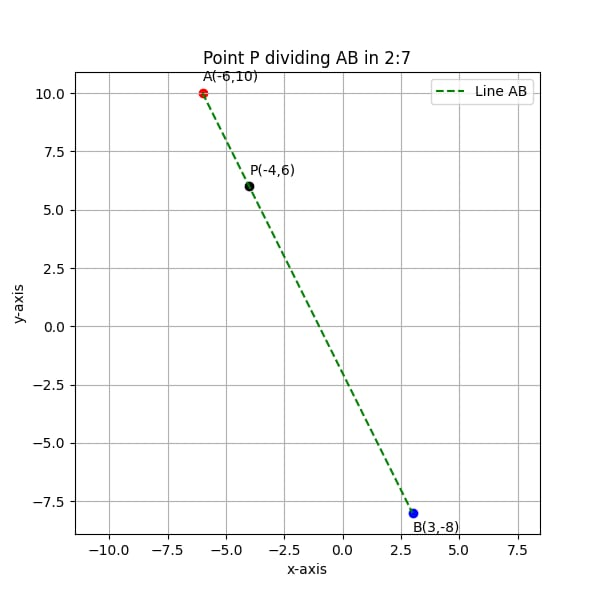
\includegraphics[width=0.7\textwidth]{figs/fig.jpg}
    \caption{Visualization of point $P(-4, 6)$ dividing the line segment joining $A(-6, 10)$ and $B(3, -8)$.}
    \label{fig:line_division}
\end{figure}

\end{document}